\chapter{Trigometric Functions}

As mentioned earlier, in a right triangle where one angle is $\theta$,
the sine of $\theta$ is the length of the side opposite $\theta$
divided by the length of the hypotenuse.

The sine function is defined for any real number. We treat that real number
$\theta$ as an angle, we draw a ray from the origin out to the unit
circle. The $y$ value of that point is the sine. So, for example,
the $\sin(\frac{4\pi}{3})$ is $-\sqrt{3}/2$

\begin{tikzpicture}[declare function={angle=240;},bullet/.style={inner
    sep=1pt,fill,draw,circle,solid}, scale=3]
    % Axis
    \draw[thick,-stealth,black] (-1.2,0)--(1.2,0) node[right] {$x$}; % x axis
    \draw[thick,-stealth,black] (0,-1.2)--(0,1.2) node[left] {$y$}; % y axis
    % Rest
    \draw (0,0) circle (1);
    \draw[thick] (0,0) -- (angle:1.0) node [midway, right] {1};
    \draw[sdkblue] (-0.1, 0.32) node[above] {$\theta = \frac{4\pi}{3}\text{ radians} = 240^\circ$};
    \draw[-stealth,sdkblue] (0.3,0) arc (0:angle:0.3);
    \draw[dashed, black] (-0.7, -0.866) -- (0.05, -0.866) node[right] {$\sin(\theta) = -\sqrt{3}/2$}; % horizontal
    \filldraw[black] (angle:1.0) circle(1pt);
\end{tikzpicture}

(Note that in this section, we will be using radians instead of
degrees unless otherwise noted. While degrees are more familiar to most
people, engineers and mathematicians nearly always use radians when
solving problems. Your calculator should have a radians mode and a
degrees mode. You want to be in radians mode.)

Similarly, we define cosine using the unit circle: to find the cosine
of $\theta$, we draw a ray from the origin at the angle $\theta$. The
$x$ component of the point where the ray intersects the unit circle is
the cosine of $\theta$.

\begin{tikzpicture}[declare function={angle=240;},bullet/.style={inner
    sep=1pt,fill,draw,circle,solid}, scale=3]
    % Axis
    \draw[thick,-stealth,black] (-1.2,0)--(1.2,0) node[right] {$x$}; % x axis
    \draw[thick,-stealth,black] (0,-1.2)--(0,1.2) node[left] {$y$}; % y axis
    % Rest
    \draw (0,0) circle (1);
    \draw[thick] (0,0) -- (angle:1.0) node [midway, right] {1};
    \draw[sdkblue] (0.1, 0.32) node[above] {$\theta = \frac{4\pi}{3}\text{ radians} = 240^\circ$};
    \draw[-stealth,sdkblue] (0.3,0) arc (0:angle:0.3);
    \draw[dashed, black]  (-0.5, -0.95) -- (-0.5, 0.05) node[left, above] {$\cos(\theta) = -0.5$}; % horizontal
    \filldraw[black] (angle:1.0) circle(1pt);
\end{tikzpicture}

From this description, it is easy to see why $\sin(\theta)^2 +
\cos(\theta)^2 = 1$. They are the legs of a right triangle with a
hypotenuse of length 1.

It should also be easy to see why $\sin(\theta) = \sin(\theta +
2\pi)$: Each time you go around the circle, you come back to where
you started.

Can you see why $\cos(\theta) = \sin(\theta + \pi/2)$? Turn the picture sideways.

\section{Graphs of sine and cosine}

Here is a graph of $y = \sin(x)$:

\begin{tikzpicture}[
tl/.style = {% tick labels
    fill=white, inner sep=1pt, font=\scriptsize,
            },                        ]
% grid
\draw[sdkblue, very thin, xstep=0.5235, ystep=0.5] (-6.6,-1.2) grid (6.6,1.2);

% y tick label
\foreach \y in {-1, -1/2, 1/2, 1}{\node[tl,left=1mm] at (0,\y) {$\y$};}
% x tick label
\foreach \x [count=\xx from -4] in 
       {-2\pi,
        -\frac{3\pi}{2},
        -\pi,           
        -\frac{\pi}{2}, 
        { },
         \frac{\pi}{2},
         \pi, 
         \frac{3\pi}{2}, 
         2\pi
        }{\node[tl,below=1mm] at (3*0.5235*\xx,0) {$\x$};}
% axes
    \draw[->,thick] (-6.5,0) -- (6.5,0) node[right] {$x$};
    \draw[->,thick] (0,-1.25) -- (0, 1.25) node[above] {$y$};
% curve
\draw[<->,thick,draw=black,
      domain=-6.5:6.5,samples=300,variable=\x] 
      plot (\x,{sin(deg{\x})});
\end{tikzpicture}

It looks like waves, right? It goes forever to the left and
right. Remembering that $\cos(\theta) = \sin(\theta + \pi/2)$, we can
guess what the graph of $y = \cos(x)$ looks like:
    
\begin{tikzpicture}[
tl/.style = {% tick labels
    fill=white, inner sep=1pt, font=\scriptsize,
            },                        ]
% grid
\draw[sdkblue, very thin, xstep=0.5235, ystep=0.5] (-6.6,-1.2) grid (6.6,1.2);

% y tick label
\foreach \y in {-1, -1/2, 1/2, 1}{\node[tl,left=1mm] at (0,\y) {$\y$};}
% x tick label
\foreach \x [count=\xx from -4] in 
       {-2\pi,
        -\frac{3\pi}{2},
        -\pi,           
        -\frac{\pi}{2}, 
        { },
         \frac{\pi}{2},
         \pi, 
         \frac{3\pi}{2}, 
         2\pi
        }{\node[tl,below=1mm] at (3*0.5235*\xx,0) {$\x$};}
% axes
    \draw[->,thick] (-6.5,0) -- (6.5,0) node[right] {$x$};
    \draw[->,thick] (0,-1.25) -- (0, 1.25) node[above] {$y$};
% curve
\draw[<->,thick,draw=black,
      domain=-6.5:6.5,samples=300,variable=\x] plot (\x,{cos(deg{\x})});
\end{tikzpicture}

\section{Plot cosine in Python}

Create a file called \filename{cos.py}:

\begin{Verbatim}
import numpy as np
import matplotlib.pyplot as plt

until = 8.0

# Make a plot of cosine
thetas = np.linspace(0, until, 32)
cosines = []
for theta in thetas:
    cosines.append(np.cos(theta))

# Plot the data
fig, ax = plt.subplots()
ax.plot(thetas, cosines, 'r.', label="Cosine")
ax.set_title("Cosine")
plt.show()
\end{Verbatim}

This will plot 32 points on the cosine wave between 0 and 8. When you
run it, you should see something like this:

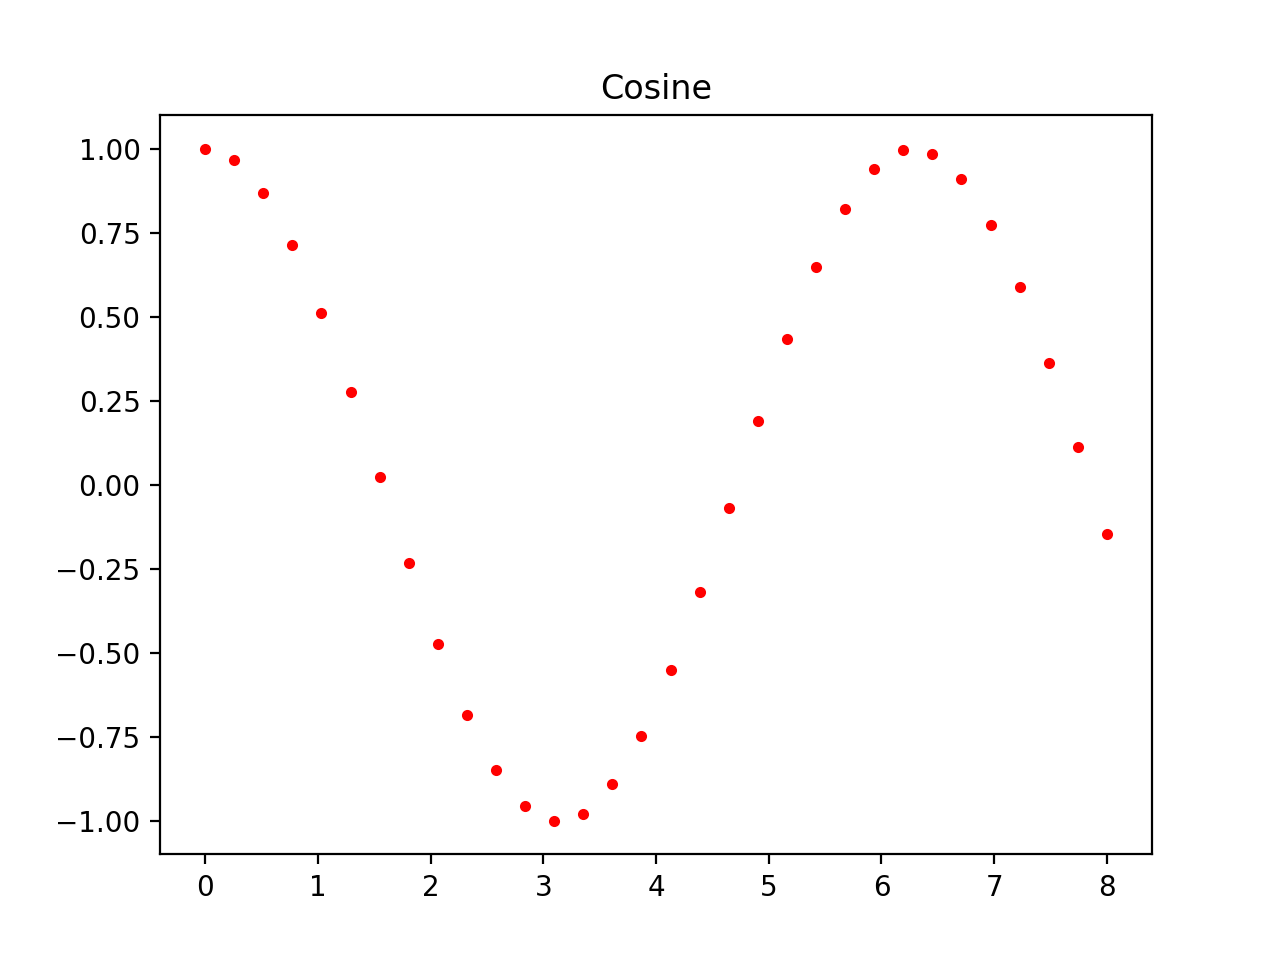
\includegraphics[width=0.8\textwidth]{cospy.png}

\section{Derivatives of sine and cos}

Here is a wonderful property of sine and cosine functions: At any point $\theta$, the slope of the sine graph at $\theta$ equals $cos(\theta)$.

For example, we know that $\sin(4\pi/3) = -(1/2)\sqrt{3}$ and
$\cos(4\pi/3) = -1/2$. If we drew a line tangent to the sine curve at
this point, it would have a slope of -1/2:

\begin{tikzpicture}[
tl/.style = {% tick labels
    fill=white, inner sep=1pt, font=\scriptsize,
            },                        ]
% grid
\draw[sdkblue, very thin, xstep=0.5235, ystep=0.5] (-1.25,-1.7) grid (6.6,1.2);

% y tick label
\foreach \y in {-3/2, -1, -1/2, 1/2, 1}{\node[tl,left=1mm] at (0,\y) {$\y$};}
% x tick label
\foreach \x [count=\xx from -1] in 
       {-\frac{\pi}{2}, 
        { },
         \frac{\pi}{2},
         \pi, 
         \frac{3\pi}{2}, 
         2\pi
        }{\node[tl,below=1mm] at (3*0.5235*\xx,0) {$\x$};}
% axes
    \draw[->,thick] (-1.25,0) -- (6.5,0) node[right] {$x$};
    \draw[->,thick] (0,-1.5) -- (0, 1.25) node[above] {$y$};
% curve
\draw[<->,thick,draw=black,
      domain=-1.75:6.5,samples=300,variable=\x] 
      plot (\x,{sin(deg{\x})});
\filldraw[black] (4.188790204786391,-0.866025403784439) circle(2pt);
\draw[->, thick, draw=red] (4.188790204786391,-0.866025403784439) -- (5.188790204786391,-1.366025403784439) node [right] {slope = -1/2} ;
\end{tikzpicture}

We say ``The derivative of the sine function is the cosine function.''

Can you guess the derivative of the cosine function? For any $\theta$, the slope of the graph of the $\cos(\theta)$ is $-\sin(\theta)$.



\section{A weight on a spring}

Let's say you fill a rollerskate with heavy rocks and attach it to the
wall with a stiff spring.  If you push the skate toward the wall a
release it, it will roll back and forth. Engineers would say ``The skate will oscillate.''

Intuitively, you can probably guess:
\begin{itemize}
\item If the spring is stronger, the skate will oscillate more times per minute.
\item If the rocks are lighter, the skate will oscillate more times per minute.
\end{itemize}

The force that the spring exerts on the skate is proportional to how
far its length is from its relaxed length. When you buy a spring, the
manufacturer advertises its ``spring rate'', which is in pounds per
inch or newtons per meter.  If a spring has a rate of 5 newtons per
meter, which means that if stretch or compress it 10 cm, it will push
back with a force of 0.5 newtons. If you stretch or compress it 20 cm,
it will push back with a force of 1 newton.

Let's write a simulation of the skate-on-a-spring. Duplicate \filename{cos.py}, and name the new copy \filename{spring.py}.  Add code to implement the simulation:

\begin{Verbatim}[commandchars=\\\{\}]
import numpy as np
import matplotlib.pyplot as plt

until = 8.0

\textbf{# Constants}
\textbf{mass = 100 # kg}
\textbf{spring_constant = -1 # newtons per meter displacement}
\textbf{time_step = 0.01 # s}

\textbf{# Initial state}
\textbf{displacement = 1.0 # height above equilibrium in meters}
\textbf{velocity = 0.0}
\textbf{time = 0.0 # seconds}

\textbf{# Lists to gather data}
\textbf{displacements = []}
\textbf{times = []}

\textbf{# Run it for a little while}
\textbf{while time <= until:}
\textbf{    # Record data}
\textbf{    displacements.append(displacement)}
\textbf{    times.append(time)}

\textbf{    # Calculate the next state}
\textbf{    time += time_step}
\textbf{    displacement += time_step * velocity}
\textbf{    force = spring_constant * displacement }
\textbf{    acceleration = force / mass}
\textbf{    velocity += acceleration}

# Make a plot of cosine
thetas = np.linspace(0, until, 32)
cosines = []
for theta in thetas:
    cosines.append(np.cos(theta))

# Plot the data
fig, ax = plt.subplots()
\textbf{ax.plot(times, displacements, 'b', label="Displacement")}
ax.plot(thetas, cosines, 'r.', label="Cosine")

\textbf{ax.set_title("Weight on Spring vs. Cosine")}
\textbf{ax.set_xlabel("Time (s)")}
\textbf{ax.set_ylabel("Displacement (m)")}
\textbf{ax.legend()}
plt.show()
\end{Verbatim}
When you run it, you should get a plot of your spring and the cosine graph on the same plot.

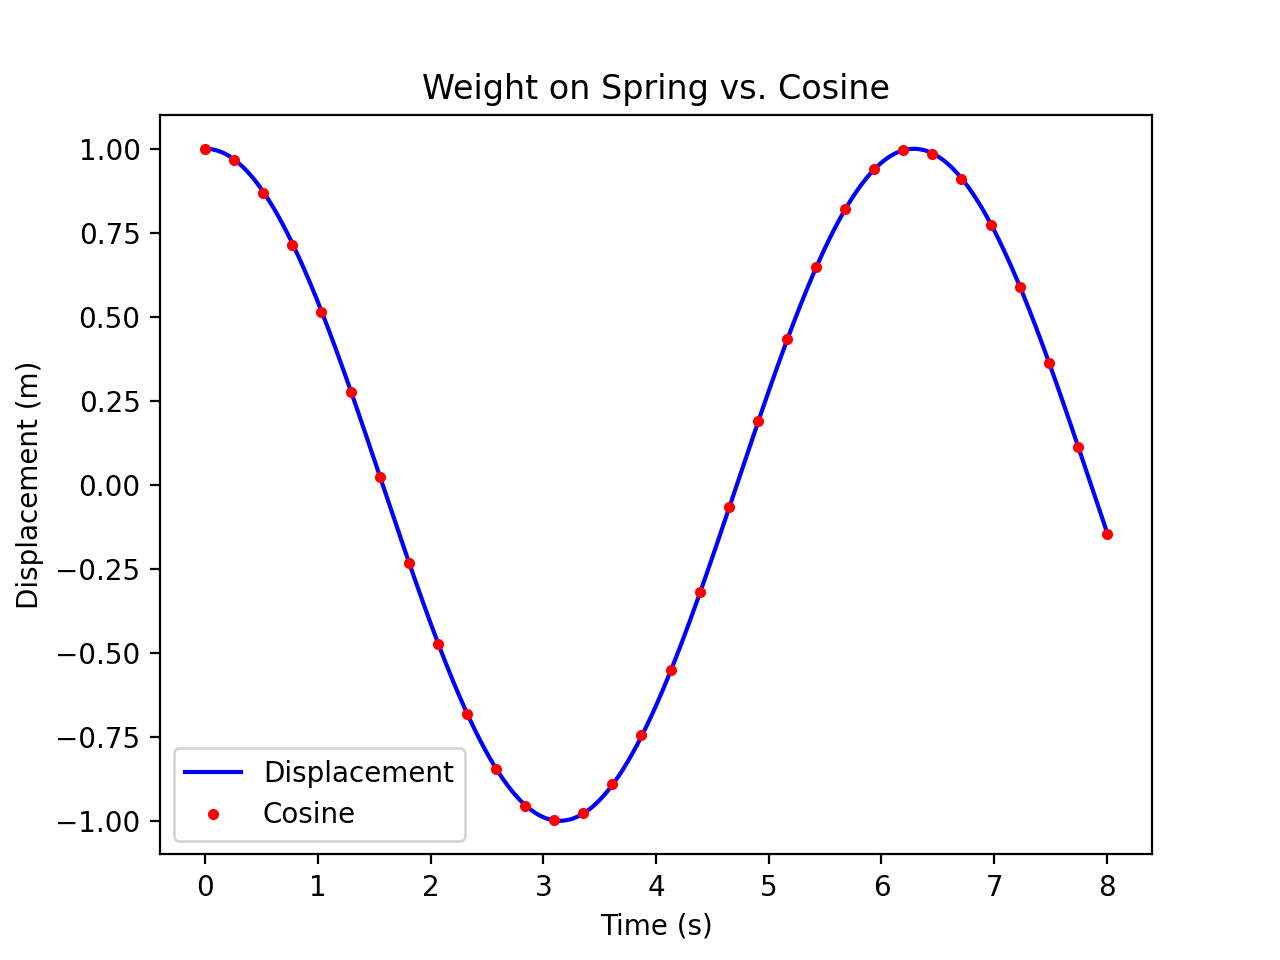
\includegraphics[width=0.8\textwidth]{springpy.png}

The position of the skate is following a cosine curve. Why?

Because a sine or cosine waves happen whenever the acceleration of 
an object is proportional to -1 times its displacement. Or in symbols:

$$a \propto - p$$

where $a$ is acceleration and $p$ is the displacement from equilibrum.

Remember that if you take the derivative of the displacement, you get
the velocity. And if you take the derivative of that, you get
acceleration. So, the weight on the spring must follow a function $f$ such that

$$f(t) \propto - f''(t)$$

Remember that the derivative of the $\sin(\theta)$ is $\cos(\theta)$.

And the derivative of the $\cos(\theta)$ is $- \sin(\theta)$

Thus these sorts of waves have an almost-magical power: their
acceleration is proportional to -1 times their displacement.

Thus sine waves of various magnitudes and frequencies are ubiquitous
in nature and technology.

\section{Integral of sine and cosine}

If we take the area between the graph and the $x$ axis of the cosine
function (and if the function is below the $x$ axis, it counts as
negative area), from 0 to $4\pi/3$, we find that it is equal to
$-(1/2)\sqrt{3}$

\begin{tikzpicture}[
tl/.style = {% tick labels                                                                                               
    fill=white, inner sep=1pt, font=\scriptsize,
            },                        ]

% y tick label                                                                                                           
\foreach \y in {-1, -1/2, 1/2, 1}{\node[tl,left=1mm] at (0,\y) {$\y$};}
% x tick label                                                                                                           
\foreach \x [count=\xx from -1] in
       {-\frac{\pi}{2},
        { },
         \frac{\pi}{2},
         \pi,
         \frac{3\pi}{2},
         2\pi
        }{\node[tl,below=1mm] at (3*0.5235*\xx,0) {$\x$};}
       % axes
       \draw[->,thick] (-1.25,0) -- (6.5,0) node[right] {$x$};
       \draw[->,thick] (0,-1.25) -- (0, 1.25) node[above] {$y$};
       % curve
       \draw[<->,thick,draw=black, domain=-1.75:6.5,samples=300,variable=\x] plot (\x,{cos(deg{\x})});
       \fill[sdkblue, domain=0:1.57,samples=100, variable=\b]
       (0, 1)
       -- plot (\b,{cos(deg(\b))})
       -- (0, 0)
       -- cycle;
       \fill[red, domain=1.57:4.188790204786391,samples=100, variable=\b]
       (1.57, 0)
       -- plot (\b,{cos(deg(\b))})
       -- (4.188790204786391, 0)
       -- cycle;
       \draw[thick, draw=black] (4.188790204786391, 1) -- (4.188790204786391,-1) node [right]{area=$-(1/2)\sqrt{3}$};
\end{tikzpicture}

We say ``The integral of the cosine function is the sine function.'' 










